\documentclass[12pt]{article}
\usepackage{hyperref,amsmath,amsfonts,fullpage,color}
\newcommand{\be}{\begin{equation}}
\newcommand{\ee}{\end{equation}}
\newcommand{\bh}{\bar{h}}
\usepackage{tikz,tkz-euclide,pgfplots}
\usetikzlibrary{arrows,positioning,fit,shapes,snakes,backgrounds,patterns,decorations.markings}

\usepackage{enumitem}
\newcounter{quesno}
\newcommand{\ques}[1]{\vspace{3em}\stepcounter{quesno}
\noindent{\bf Question \thequesno.} \emph{(#1 points)\\}
}
\begin{document}

\begin{center}

{\bf\Large General Relativity}

\vspace{1em}
{\bf\large Final Examination, 17${}^{\text{th}}$ Jan 2020}

\vspace{1em}
{\bf Time:} 4 hours


\end{center} 
\vspace{1em}
{\bf\Large\noindent Name:}

\vspace{1em}
\hrule
\vspace{1em}
\noindent
{\bf Instructions:} 
This is an oral exam with written preparation: during the oral exam, I will look through your notes and ask for additional explanations. As soon as you have finished preparing any one question, you can start the oral exam with
that question. For full marks, all questions must be solved.

\vspace{1em}
\hrule

\ques{2} 
The components of the Riemann tensor in some coordinates are $R^\mu{}_{\nu\rho\sigma}$.
Write down how they transform under a change of coordinates.
Define the Ricci tensor by $R_{\mu\nu} = R^\rho{}_{\mu\rho\nu}$, and show explicitly that this transforms as a tensor under change of coordinates.

\vspace{1em}

\color{red}
\noindent {\bf Solution:}
Recall that upper indices transform like $dx^{\prime \mu} = \frac{\partial x^{\prime \mu}}{\partial x^\rho} dx^\rho$ and lower indices in the opposite way. 
So, 
\be
R^{\prime \mu}{}_{\nu\rho\sigma}
= 
\frac{\partial x^{\prime \mu}}{\partial x^\kappa} \frac{\partial x^\lambda}{\partial x^{\prime \nu}} \frac{\partial x^\alpha}{\partial x^{\prime \rho}} \frac{\partial x^\beta}{\partial x^{\prime \sigma}} 
R^{\kappa}{}_{\lambda\alpha\beta}
\ee
Then,
\be
R^{\prime \mu}{}_{\nu\mu\sigma}
= 
\frac{\partial x^{\prime \mu}}{\partial x^\kappa} \frac{\partial x^\lambda}{\partial x^{\prime \nu}} \frac{\partial x^\alpha}{\partial x^{\prime \mu}} \frac{\partial x^\beta}{\partial x^{\prime \sigma}} 
R^{\kappa}{}_{\lambda\alpha\beta}= 
\delta_\kappa^\alpha  \frac{\partial x^\lambda}{\partial x^{\prime \nu}} \frac{\partial x^\beta}{\partial x^{\prime \sigma}} R^{\kappa}{}_{\lambda\alpha\beta}
= 
  \frac{\partial x^\lambda}{\partial x^{\prime \nu}} \frac{\partial x^\beta}{\partial x^{\prime \sigma}} 
R^{\kappa}{}_{\lambda\kappa\beta}
\ee
so the Ricci tensor is also a tensor.

\color{black}

\ques{3}
Consider a manifold on which we have both a metric, $g_{\mu\nu}$, and a totally antisymmetric $(0,3)$ tensor, $H_{\mu\nu\rho} = H_{[\mu\nu\rho]}$.
We can define a connection with components $\hat\Gamma_{\mu\nu}{}^\rho$ by:
\be
\hat \Gamma_{\mu\nu}{}^\rho = \Gamma_{\mu\nu}{}^\rho + \frac{1}{12} g^{\rho \sigma} H_{\mu\nu\sigma}
\label{stringconn}
\ee
where $\Gamma_{\mu\nu}{}^\rho$ denotes the components of the usual Levi-Civita connection.

\begin{enumerate}[label=\alph*)]
\item (\emph{2 points}) Is the new connection $\hat\Gamma_{\mu\nu}{}^\rho$ defined in equation \eqref{stringconn} torsion-free? Is it metric compatible? 
\item (\emph{1 point}) Show that the geodesics of the connection $\hat\Gamma_{\mu\nu}{}^\rho$ are the same as the geodesics of the Levi-Civita connection. 
\end{enumerate}


\color{red}
\noindent {\bf Solution:}
\begin{enumerate}[label=\alph*)]
\item Torsion-free: $\Gamma_{[\mu\nu]}{}^\rho = 0$. Metric compatible: $\nabla_\mu g_{\nu\rho} = 0$.
\item It is not torsion-free, $\hat\Gamma_{[\mu\nu]}{}^\rho = \frac{1}{12} g^{\rho\sigma} H_{\mu\nu\sigma}$. 
Metric compatibility:
\be
\begin{split} 
\hat\nabla_\mu g_{\nu\rho}  & = 
\partial_\mu g_{\nu\rho} - \Gamma_{\mu\nu}{}^\sigma g_{\sigma \rho} - \Gamma_{\mu\rho}{}^\sigma g_{\nu\sigma} 
- \frac{1}{12} H_{\mu \nu \lambda} g^{\sigma \lambda} g_{\sigma \rho} 
- \frac{1}{12} H_{\mu \rho \lambda} g^{\sigma \lambda} g_{\sigma \nu} 
\\ & 
= - \frac{1}{12} H_{\mu \nu \rho}  
- \frac{1}{12} H_{\mu \rho \nu} 
= 0 
\end{split} 
\ee
\item The geodesic equation is
\be
\frac{d^2x^\mu}{d\lambda^2} + \hat \Gamma_{\nu\rho}{}^\mu \frac{dx^\nu}{d\lambda} \frac{dx^\rho}{d\lambda} = 0 
\ee
so only the symmetric part of the connection contributes; $\hat\Gamma_{[\nu\rho]}{}^\mu = \Gamma_{\nu\rho}{}^\mu$
\end{enumerate}
\color{black}



\ques{4}
The Schwarzschild metric is:
\be
ds^2 = - f(r) dt^2 + f(r)^{-1} dr^2 + r^2 d \theta^2 + r^2 \sin^2 \theta d\phi^2 
\ee
where $f(r) = 1 - \frac{2GM}{r}$. 

\begin{enumerate}[label=\alph*)]
\item  (\emph{2 points}) Suppose you are sufficiently interested in physics that you decide to fall into a Schwarzschild black hole to see what happens. 
Your friends and family think this might be unsafe, as they have noticed there are singularities in the Schwarzschild metric. 
Where do these singularities occur, which should you be genuinely concerned about, and why? 
\item (\emph{2 points}) Determine the Schwarzschild metric in the ingoing Eddington-Finkelstein coordinates $(v,r,\theta,\phi)$, where
\be
v = t + r + 2GM \ln\left| \frac{r}{2GM} - 1 \right|
\ee
and explain how this supports your answer to part a). 
\end{enumerate} 

{\color{red} {\bf Solution}

\begin{enumerate}[label=\alph*)]
\item $r=2GM$ is a coordinate singularity, it is an artefact of the coordinate system, while $r=0$ is a curvature singularity; scalars built from the curvature blow up, this is a genuine singularity of the manifold.
\item We have
\be
\begin{split}
dv & = dt + dr + \frac{2GM}{\frac{r}{2GM} - 1} \frac{dr}{2GM} = dt + dr \left( 1 + \frac{1}{\frac{r}{2GM} - 1} \right)
\\ &  = dt + dr \left( \frac{ \frac{r}{2GM} }{ \frac{r}{2GM} -1}\right) 
\\ & = dt + \frac{dr}{1-\frac{2GM}{r}}
\end{split}
\ee
Hence
\be
-\left(  1 - \frac{2GM}{r} \right) dt^2 = -\left(  1 - \frac{2GM}{r} \right) dv^2 + 2 dv dr - \frac{dr^2}{1- \frac{2GM}{r}}
\ee
so
\be
ds^2 = -\left(  1 - \frac{2GM}{r} \right) dv^2 + 2 dv dr + r^2 d \theta^2 + r^2 \sin^2 \theta d\phi^2 
\ee
There is no singularity at $r=2GM$.
\end{enumerate}
}


\ques{5}
The metric of de Sitter is:
\be
ds^2 =- dt^2 +  L^2  \cosh^2 (t/L) \left( d\chi^2 + \sin^2 \chi \left( d\theta^2 + \sin^2\theta d\phi^2 \right)\right)  \,.
\label{dsmetric} 
\ee
where $t \in (-\infty, \infty)$, $\chi \in (0,\pi)$ and $(\theta,\phi)$ are the usual coordinates on a two-sphere (and together $\chi, \theta,\phi$ parametrise a three-sphere).

\begin{enumerate}[label=\alph*)]
\item (\emph{2 points})  Explain why this metric is a candidate cosmological solution that could describe our universe. What is the scale factor?  
\item (\emph{1 point}) Explain why two metrics that are related by $g_{\mu\nu} = \Omega^2 \bar g_{\mu\nu}$, can be said to have the same causal structure. 
\item (\emph{2 points}) For de Sitter, make the coordinate transformation
\be
\cosh \frac{t}{L} = \frac{1}{\cos \eta} \,,
\ee
and draw the Penrose diagram. 

\end{enumerate}


\color{red}
{\bf Solution}
\begin{enumerate}[label=\alph*)]
\item The spatial part is expanding with scale factor $a(t) = L^2 \cosh^2 (t/L)$, and for constant $t$, spatial slices are homogeneous and isotropic, in accord with observation. 
\item Null geodesics/lightcones are the same in each other. 
\item 
One has
\be
\sinh \frac{t}{L} \frac{dt}{L} = - \frac{\sin \eta}{\cos^2 \eta} d \eta 
\ee
\be
\Rightarrow dt^2 = \frac{L^2}{\cos^4 \eta} \frac{\sin^2 \eta}{\sinh^2 \frac{t}{L}} = \frac{L^2}{\cos^4 \eta} \frac{\sin^2 \eta}{\cosh^2 \frac{t}{L} - 1}
=  \frac{L^2}{\cos^4 \eta} \frac{\sin^2 \eta}{\frac{1-\cos^2 \eta}{\cos^2 \eta}}
\ee
\be
\Rightarrow dt^2 = \frac{L^2}{\cos^2 \eta} 
\ee
using
\be
\cosh^2 - \sinh^2 = 1 \,,\quad \cos^2 + \sin^2 = 1 
\ee
and hence 
\be
ds^2 = \frac{L^2}{\cos^2 \eta} \left( - d\eta^2 + d\chi^2 + \sin^2 \chi \left( d\theta^2 + \sin^2\theta d\phi^2 \right) \right)
\ee
This is conformal to:
\be
d\hat s^2 = 
 - d\eta^2 + d\chi^2 + \sin^2 \chi \left( d\theta^2 + \sin^2\theta d\phi^2 \right)
\ee
with $\eta \in (-\pi/2,\pi/2)$ i.e. from $\cos \eta = -1$ at $t=-\infty$ to $\cos \eta = -1$ at $t=+\infty$ and $\chi \in (0,\pi)$
The Penrose diagram is a square:
\color{black}

\begin{figure}[ht]
\centering
\begin{tikzpicture}
\tikzset{->-/.style={decoration={
  markings,
  mark=at position 0.5 with {\arrow{>}}},postaction={decorate}}}


\draw (-2,0) node [below] {$\chi=0$} -- (-2,4) node [left] {$\eta = +\frac{\pi}{2}$};
\draw (-2,4) -- (2,4);
\draw (-2,0) node [left] {$\eta = -\frac{\pi}{2}$} -- (2,0);
\draw (2,0) node [below] {$\chi=\pi$}  -- (2,4);

\draw [red,thick,->-] (-1,0) -- (2,3);
\draw [red,thick,->-] (2,3) -- (1,4);

\end{tikzpicture}
\caption{Penrose diagram of de Sitter}
\label{pends} 
\end{figure}

\begin{figure}[ht]
\centering
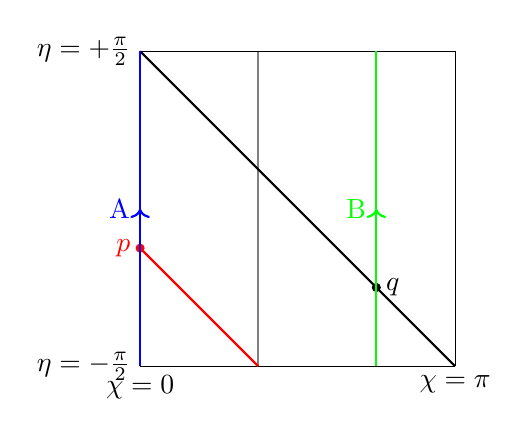
\begin{tikzpicture}
\tikzset{->-/.style={decoration={
  markings,
  mark=at position 0.5 with {\arrow{>}}},postaction={decorate}}}

%\draw[pattern=crosshatch dots, pattern color=black] (-2,0) -- (2,0) -- (-2,4) -- (-2,0);
%\draw[pattern=north west lines, pattern color=red] (-2,0) -- (-0.5,0) -- (-2,1.5) -- (-2,0);
\draw[color=gray,thick] (-0.5,0) -- (-0.5,4);

\draw (-2,0) node [below] {$\chi=0$} -- (-2,4) node [left] {$\eta = +\frac{\pi}{2}$};
\draw (-2,4) -- (2,4);
\draw (-2,0) node [left] {$\eta = -\frac{\pi}{2}$} -- (2,0);
\draw (2,0) node [below] {$\chi=\pi$}  -- (2,4);


\draw [thick] (2,0) -- (-2,4);

\draw [thick,red] (-2,1.5) -- (-0.5,0);
\filldraw [red] (-2,1.5) circle (0.05cm) node [left] {$p$};

\filldraw [black] (1,1) circle (0.05cm) node [right] {$q$};


\draw [blue,thick,->-] (-2,0) -- (-2,4) node [left,midway] {A};

\draw [green,thick,->-] (1,0) -- (1,4) node [left,midway] {B};

\end{tikzpicture}
\caption{Horizons in de Sitter: the black line is the cosmological horizon of the observer $A$, and the vertical gray line is the particle horizon at $p$.}
\label{pendshor} 
\end{figure}
\end{enumerate}
\color{black}

\ques{6}
The linearised Einstein equation is
\be
- \frac{1}{2} \partial^\rho\partial_\rho \bh_{\mu\nu} + \partial^\rho \partial_{(\mu} \bh_{\nu)\rho}
- \frac{1}{2} \eta_{\mu\nu} \partial^\rho \partial^\sigma \bh_{\rho\sigma} = 8 \pi G T_{\mu\nu} \,,
\ee
when written in terms of $\bh_{\mu\nu} = h_{\mu\nu} - \frac{1}{2} h \eta_{\mu\nu}$. 

\begin{enumerate}[label=\alph*)]
\item (\emph{1 point}) By making an appropriate gauge choice, explain why the linearised Einstein equation leads to \emph{gravitational waves}.
\item (\emph{2 point}) Consider an experiment involving two freely falling test particles, arranged so that one is at spatial position $x^i = (0,0,0)$ and the other at spatial position $x^i=(L_x,0,0)$.
Suppose a gravitational wave travelling along the $z$-axis passes through the laboratory, corresponding to the following metric perturbation:
\be
h_{\mu\nu} = \begin{pmatrix}
0 & 0 & 0 & 0 \\
0 & h_{+}(t-z) & 0 & 0 \\
0 & 0 & - h_{+}(t-z) & 0 \\
0 & 0 & 0 & 0
\end{pmatrix} \,.
\ee
Show that the proper distance between the test particles is given by: 
\be
\Delta s \approx L_x \left( 1 + \frac{1}{2} h_{+}(t) \right) \,.
\ee
If a third test particle is introduced at $x^i=(0,L_y,0)$ show that the proper distance between it and the particle at the origin is
\be
\Delta s \approx L_y \left( 1 - \frac{1}{2} h_{+}(t) \right) \,.
\ee
\item (\emph{3 points}) Consider a binary system consisting of two massive bodies in a circular orbit, which are emitting gravitational waves.
Explain \emph{qualitatively} what happens to the system, and sketch the corresponding gravitational wave signal which would be observed by a detector such as LIGO.
You should mention the following terms: \emph{inspiral}, \emph{merger}, \emph{ringdown}, explain how the interferometer detects a wave such as that described in part b), and connect the features of the signal to the physics of the binary pair. 

\end{enumerate}
\color{red}
{\bf Solution}
\begin{enumerate}[label=\alph*)]
\item The gauge choice $\partial^\nu \bh_{\mu\nu} = 0$ gives a wave equation: $\partial^\rho\partial_\rho \bh_{\mu\nu} = - 16 \pi G T_{\mu\nu}$, whose solutions are waves.
\item For the first case
\be
\begin{split} 
\Delta s = \int_0^{L_x} \sqrt{ds^2} & = \int_0^{L_x} \sqrt{g_{\mu\nu} dx^\mu dx^\nu} \\
 & = \int_0^{L_x} dx \sqrt{g_{xx}} \\
 & = \int_0^{L_x} dx \sqrt{1+h_{+}(t)}\\
 & \approx {L_x} \left( 1 + \frac{1}{2} h_{+}(t) \right) \,.
\end{split}
\ee
For the second case
\be
\begin{split} 
\Delta s = \int_0^{L_y} \sqrt{ds^2} & = \int_0^L \sqrt{g_{\mu\nu} dx^\mu dx^\nu} \\
 & = \int_0^{L_y} dy \sqrt{g_{yy}} \\
 & = \int_0^{L_y} dy \sqrt{1-h_{+}(t)}\\
 & \approx {L_y} \left( 1 - \frac{1}{2} h_{+}(t) \right) \,.
\end{split}
\ee
\item As they orbit they emit gravitational radiation and so lose energy.
As they lose energy, their separation decreases, and their angular velocity increases.
Finally they reach each other and merge into a single object.

The gravitational wave signal consists of a wave whose frequency is related to the angular velocity of the orbiting body, in fact $\Omega_{GW} = 2 \Omega$.
This frequency varies in time, and increases during \emph{inspiral} as the bodies come closer together, before peaking at the \emph{merger}, and dropping off in the \emph{ringdown} phase post-merger. 

The effect of the wave is to alter the proper distances along which light on two orthogonal arms travel; hence light that is perfectly in sync initially will travel different distances before being detected. This leads to a phase shift and an interference pattern from which we can discern the difference in distance. 
This gives the following measurement:

\begin{figure}[h]
\centering
\begin{tikzpicture}
\begin{axis}[
  axis x line=bottom,    
  %ymin=-15000,ymax=15000,xmax=4,
  %ymin=-110,ymax=110,xmax=60,
  ymin = -1.3,ymax=1.3,
  axis y line=center,
  xlabel={Time},
  ylabel={},
  ylabel near ticks,
  xlabel style={below},
  ylabel style={},
  xtick style={draw=none},
  ytick = {0},scaled ticks=false,
  xticklabels={,,}
black,
%width=16cm,height=5cm
,thick] 
%\addplot[domain=0:55,samples=800, thick, red,]{(x/5-1)*(x/5-1)*cos(pow(x,2) - x)};
\addplot[red,thick] table {../../Notes/waveform.dat};
%\addplot[domain=0:0.3,samples=800, thick, red,]{(( 1-x )^(-3/4))*cos(2*x*( 1-x )^(-3/8))};
\end{axis}

\draw (0,5) node [left] {$h\sim\frac{\delta L}{L}$};

\draw (2.5,6) node [above] {\small Inspiral};
%\draw (0,6) -- (5.3,6) node [above,midway] {Inspiral};
%\draw (0,5.8) -- (0,6.2);
%\draw (5.3,5.8) -- (5.3,6.2);

%\draw (5.4,5.8) -- (5.4,6.2);
%\draw (5.8,5.8) -- (5.8,6.2);

\draw (5.5,6) node [above] {\small Merger};

\draw (6.8,5.5) node [above] {\small Ringdown};

\end{tikzpicture}
\end{figure}

Assuming a Newtonian analysis, we can use Kepler's law to relate the angular frequency and radial separation. If we know the angular frequency at the merger, i.e. the maximum value, we know the minimum value of the separation prior to merger. This allows us to bound the compactness of the system.
Also knowing frequency and its rate of change lets us determine (roughly) the mass of the system, and the overall amplitude then lets us determine the distance to the source.


\end{enumerate}
\color{black}


\end{document}
